\documentclass[tikz,border=4pt]{standalone}
\usepackage{amsmath,amssymb,bm,setspace}
\usepackage{tikz,pgfplots}
\pgfplotsset{compat=1.18}
\usetikzlibrary{arrows.meta,calc,positioning,decorations.pathreplacing}
\begin{document}
% Case-D tangential lever variation for both directions of the achieved
% angular offset about t_1. Error bars show the sample standard deviation of the three
% repetitions at each setting.
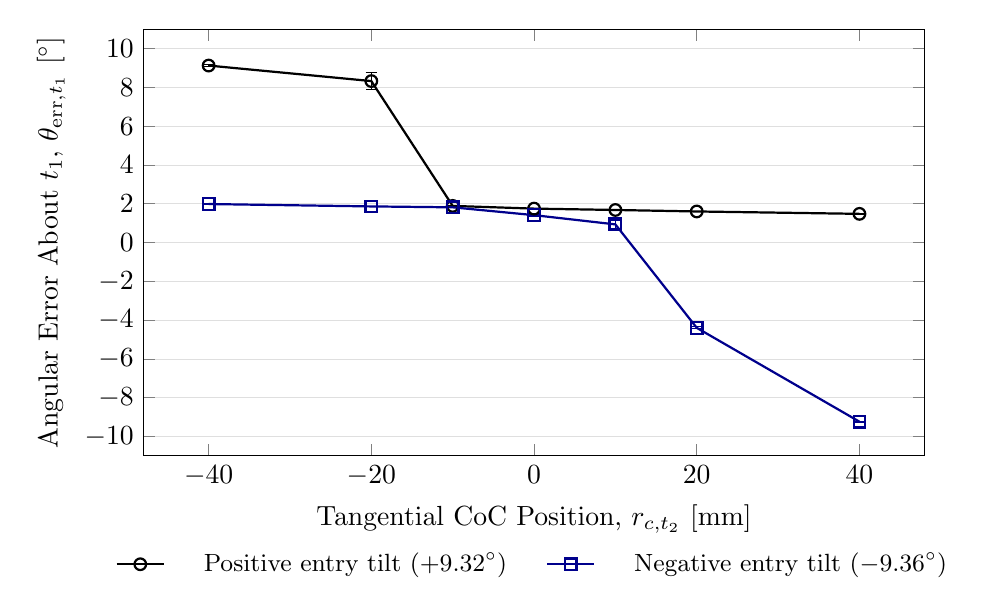
\begin{tikzpicture}
\pgfplotsset{
  every axis/.append style={
    width=11.5cm, height=7.0cm,
    xmin=-48, xmax=48, ymin=-11, ymax=11,
    xtick={-40,-20,0,20,40},
    ytick={-10,-8,-6,-4,-2,0,2,4,6,8,10},
    ymajorgrids=true,
    xmajorgrids=false,
    grid style={gray!25, very thin},
    tick label style={font=\normalsize},
    label style={font=\normalsize},
    legend style={font=\small, draw=none, fill=none,
                  cells={anchor=west}, at={(0.5,-0.20)}, anchor=north,
                  legend columns=2, column sep=1.2em},
    every axis plot/.append style={thick, mark size=2.1pt},
  },
}
\begin{axis}[
    xlabel={Tangential CoC Position, \(r_{c,t_2}\) [mm]},
    ylabel={Angular Error About \(t_1\), \(\theta_{\mathrm{err},t_1}\) [\(^\circ\)]},
  ]
\addplot[black, mark=o, mark options={fill=white},
         error bars/.cd, y dir=both, y explicit] coordinates {
  (-40,9.126666667) +- (0,0.070237692)
  (-20,8.326666667) +- (0,0.423595719)
  (-10,1.890000000) +- (0,0.010000000)
  (0,1.750000000) +- (0,0.000000000)
  (10,1.680000000) +- (0,0.010000000)
  (20,1.603333333) +- (0,0.005773503)
  (40,1.480000000) +- (0,0.010000000)};
\addlegendentry{Positive entry tilt \((+9.32^\circ)\)}
\addplot[blue!55!black, mark=square, mark options={fill=white},
         error bars/.cd, y dir=both, y explicit] coordinates {
  (-40,1.986666667) +- (0,0.020816660)
  (-20,1.863333333) +- (0,0.011547005)
  (-10,1.816666667) +- (0,0.011547005)
  (0,1.413333333) +- (0,0.056862407)
  (10,0.936666667) +- (0,0.214553801)
  (20,-4.396666667) +- (0,0.055075705)
  (40,-9.236666667) +- (0,0.030550505)};
\addlegendentry{Negative entry tilt \((-9.36^\circ)\)}
\end{axis}
\end{tikzpicture}

\end{document}
